\StartOf{Lecture 18}

\Today{(1) Source Coding \& Entropy, (2) Joint / Conditional Entropy, (3) Entropy Rate, (4) Source Coding Theorem}

\announcements{
\begin{itemize}
  \item Today's reading: Claude E. Shannon, ``A Mathematical Theory of Communication'', \emph{The Bell System Technical Journal}, 1948.  Read Part I.
\end{itemize}
}

\section{Source Coding}

We talk in this course quite a bit about ``bits'', the fundamental measure of the information we're designing a communication system to send.  The purpose of today's lecture is to describe what a \emph{bit rate} really means when we know what kind of data will be sent (a.k.a. our ``source'').  The short story is, when we do know about the data being sent, that the data rate we need to send is \emph{at least} the \emph{entropy rate} of the data, which is a quantity that can be determined from the statistics of the data.

This topic is a semester-long course at the graduate level in
itself; but the basic ideas can be presented pretty quickly.  Claude Shannon presented an introduction to source coding in Part 1 of his 1948 paper, ``A mathematical theory of communication'' \cite{shannon1948mathematical}, which introduced the concept.

We have done a lot of counting of bits as our primary measure of
communication systems.  Our information source is measured in bits,
or in bits per second.  Modulation schemes' bandwidth efficiency is
measured in bits per Hertz, and energy efficiency is energy per bit
over noise PSD.  Lots of what a communication engineer does is measured in bits!

But how do we measure the bits of a source (\eg, audio, video, email, SMS, $\ldots$)?  Information can often be represented in many different ways. Images and sound can be encoded in different ways.  Text files can be presented in different ways.

Here are two misconceptions:
\begin{enumerate}
  \item The file size tells you how much information is contained within the file.
  \item The number of bits is the $\log_2$ of the number of different values the data could possibly send.
\end{enumerate}

For example, consider a digital black \& white image (not grayscale, in this example, truly black or white).
\begin{enumerate}
  \item You could store it as the value for each pixels.  Each pixel has two
  possibilities (possible values),
  thus we could encode it in $\log_2 2 = 1$ bit per pixel.
  \item You could simply send the coordinates of the pixels of one
  of the colors (\eg all black pixels).
\end{enumerate}
How many bits would be used in these two representations? What would
make you decide which one is more efficient?

\vspace{0.05in} \noindent  From this example, two equivalent representations could require a different number of bits.  This is the idea behind \emph{source compression}. For example, .zip or .tar files represent the exact same information that was contained in the original files, but with fewer bits.

\vspace{0.05in} \noindent  What if we had a fixed number of bits to
send any image, and we used the sparse B\&W image coding scheme (2.)
above?  Sometimes, the number of bits in the compressed image would
exceed what we had allocated.  This would introduce errors into the
image.

Two types of compression algorithms:
\begin{itemize}
  \item Lossless: \eg, Zip or compress.
  \item Lossy:  \eg, JPEG, MP3, MP4
\end{itemize}

\Note{Both ``zip'' and the linux ``compress'' commands use the
Lempel-Ziv algorithm for source compression.}

So what is the intrinsic measure of bits of text, an image, audio, or video?

\subsection{Entropy}

Entropy is a measure of the randomness of a random variable (r.v.).
\emph{Randomness} and \emph{information}, in non-technical language,
are just two perspectives on the same thing:
\begin{itemize}
  \item If you are told the value of a r.v.\ that doesn't vary that
    much, that telling conveys very little information to you.
  \item If you are told the value of a very ``random'' r.v., that
    telling conveys quite a bit of information to you.
\end{itemize}

Our technical definition of entropy of a discrete random variable is as
follows.

\Definition{Entropy}{ Let $X$ be a discrete random variable with pmf
$p_X(x_i) = \PR{X=x}$.  Here, there is a finite or countably
infinite set $S_X$, and $x \in S_X$.   We will shorten the notation
by using $p_i$ as follows:
\[
  p_i = p_X(x_i) = \PR{X=x_i}
\]
where $\{x_1, x_2, \ldots\}$ is an ordering of the possible values
in $S_X$. Then the entropy of $X$, in units of bits, is defined as,
\begin{equation} \label{E:Entropy}
  \entropy{X} = -\sum_i p_i \log_2 p_i   %= \sum_i p_i \log_2 \frac{1}{p_i}
\end{equation}
}

Notes:
\begin{itemize}
  \item $\entropy{X}$ is an operator on a random variable, not a function of a random variable.
    It returns a (deterministic) number, not another random variable.  This it is like
    $\E{}{X}$, another operator on a random variable.
  \item Entropy of a discrete random variable $X$ is calculated using the
    probability values of the pmf of $X$, $p_i$.  Nothing else is needed.
  \item The sum will be from $i=1\ldots N$ when $|S_X| = N < \infty$.
  \item Use that $0 \log 0 = 0$.  This is true in the limit of $x \log x$
    as $x \rightarrow 0^+$.
  \item All ``log'' functions are log-base-2 in information theory
    unless otherwise noted. Keep this in mind when reading a book on information theory.
  The ``reason'' the units are bits is because of the base-2 of the log.
   Actually, when theorists use $\log_e$ or the natural log, they express information in ``nats'', short for ``natural'' digits.
\end{itemize}

\Example{Binary r.v.} A binary (Bernoulli) r.v.\ has pmf,
\[
  p_X(x) = \pdfarrays{s}{x=1}{1-s}{x=0}
\]
What is the entropy $\entropy{X}$ as a function of $s$?

\Solution{ Entropy is given by (\ref{E:Entropy}) and is:
\[
  H[X] = - s \log_2 s - (1-s) \log_2 (1-s)
\] }
The solution is plotted in Figure \ref{F:EntropyBinaryRV}.

\begin{figure}[htbp]
  \centerline{  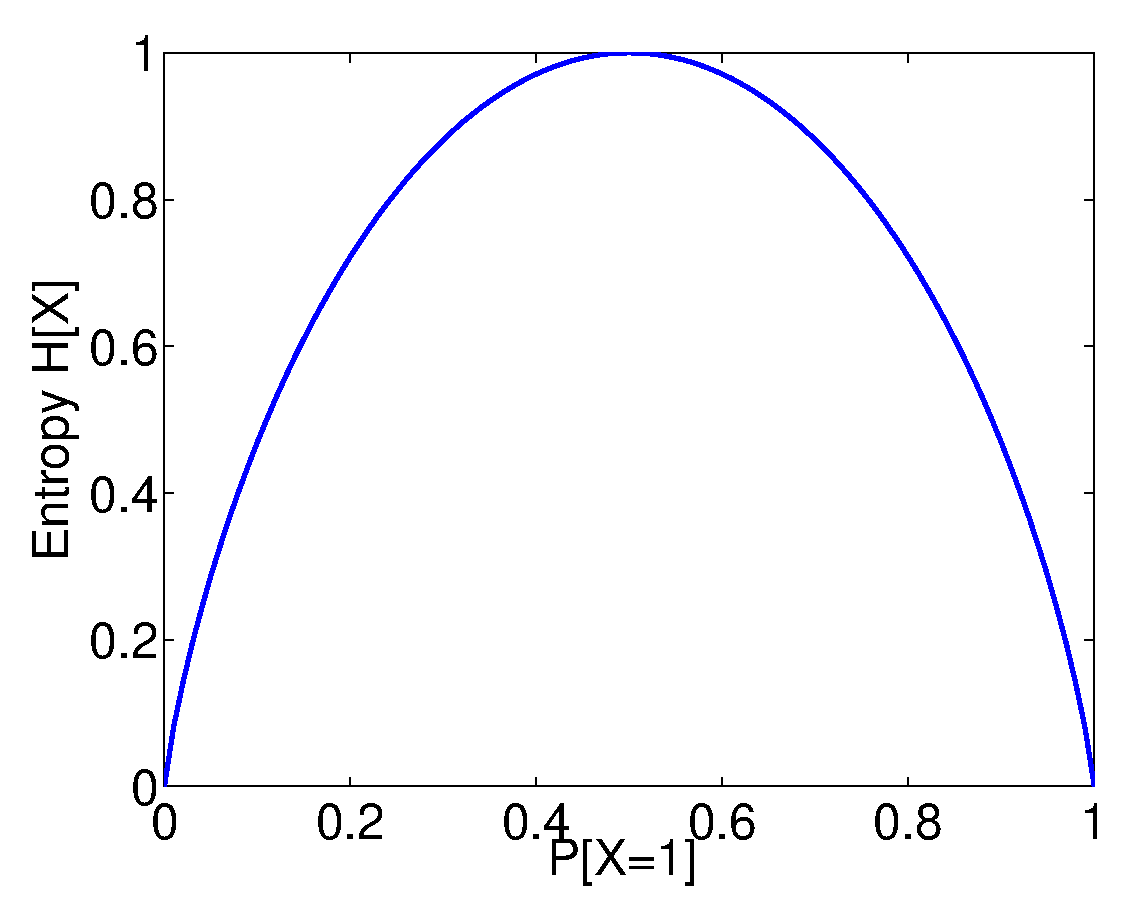
\includegraphics[width=2.5in]{../images/plotEntropyBinaryRV.eps}  }
  \caption{Entropy of a binary r.v.}
  \label{F:EntropyBinaryRV}
\end{figure}

\Example{Non-uniform source with five messages}  Some signals are
more often close to zero (\eg, audio).  Model the r.v.\ $X$ to have
pmf,
\[
p_X(x) = \left\{\begin{array}{ll} 1/16, & x=2 \\
                                  1/4, & x=1 \\
                                  1/2, & x=0 \\
                                  1/8, & x=-1 \\
                                  1/16, & x=-2 \\
                                  0, & o.w. \end{array}\right.
\]
What is its entropy $\entropy{X}$?

\Solution{
\begin{eqnarray}
 \entropy{X} &=& \frac{1}{2} \log_2 2 + \frac{1}{4} \log_2 4 + \frac{1}{8} \log_2 8 + 2 \frac{1}{16} \log_2 16
     \nonumber \\
   &=& \frac{15}{8} \mbox{ bits}
\end{eqnarray}
}

How could you encode $X$ to have an average of $15/8$ bits per value of $X$?

\Solution{
Generally we want to use fewer bits when the value is more likely:
\begin{itemize}
    \item ``2'': encode as 1110
    \item ``1'': encode as 10
    \item ``0'': encode as 0
    \item ``-1'': encode as 110
    \item ``-2'': encode as 1111
\end{itemize}
For example, if we observe $1101110000$ we would know the true values would be $-1, 2, 0,0,0$.  On average the encoding would take 
\[
\mbox{bits per }X = \frac{1}{2} 1 + \frac{1}{4} 2 + \frac{1}{8} 3 + 2 \frac{1}{16} 4 = \frac{15}{8} \mbox{ bits}
\]
}

Other questions:
\begin{enumerate}
  \item Do you need to know what the symbol set $S_X$ is?
  \item Would multiplying $X$ by 2 change its entropy?
  \item Would an arbitrary one-to-one function change the entropy of $X$?
\end{enumerate}

\subsection{Joint Entropy}

\Definition{Joint Entropy}{ The joint entropy of two random
variables $X_1, X_2$ with event sets $S_{X_1}$ and $S_{X_2}$ is
defined as
\begin{equation} \label{E:JointEntropy}
  H[X_1, X_2] = - \sum_{x_1 \in S_{X_1}} \sum_{x_2 \in S_{X_2}}
     p_{X_1,X_2}(x_1, x_2) \log_2 p_{X_1,X_2}(x_1, x_2)
\end{equation}
 }

For $N$ joint random variables, $X_1, \ldots, X_N$, entropy is
\[
  H[X_1, \ldots, X_N] = - \sum_{x_1 \in S_{X_1}} \cdots \sum_{x_N \in S_{X_N}}
     p_{X_1, \ldots, X_N}(x_1, \ldots, x_N) \log_2 p_{X_1, \ldots, X_N}(x_1, \ldots, x_N)
\]

What is the entropy for $N$ i.i.d. random variables?  You can show
that
\[
  H[X_1, \ldots, X_N] = - N \sum_{x_1 \in S_{X_1}} p_{X_1}(x_1) \log_2
  p_{X_1}(x_1) = N H(X_1)
\]
The entropy of $N$ i.i.d. random variables has $N$ times the entropy
of any one of them.  In addition, the entropy of any $N$ independent
(but possibly with different distributions) r.v.s is just the sum of
the entropy of each individual r.v.

When r.v.s are not independent, the joint entropy of $N$ r.v.s is
less than $N$ times the entropy of one of them.  Intuitively, if you
know some of them, because of the dependence or correlation, the
rest that you don't know become less informative.  For example, the
B\&W image, since pixels are correlated in space, the joint r.v.\ of
several neighboring pixels will have less entropy than the sum of
the individual pixel entropies.

\subsection{Conditional Entropy}

How much additional entropy is in the joint random variables $X_1,
X_2$ compared just to one of them?  This is often an important
question because it answers the question, ``How much additional
information do I get from both, compared to just one of them?''.  We
call this difference the conditional entropy, $H[X_2 | X_1]$:
\begin{equation} \label{E:ConditionalEntropy}
  H[X_2 | X_1] = H[X_2, X_1] - H[X_1].
\end{equation}
What is an equation for $H[X_2 | X_1]$ as a function of the joint
probabilities $p_{X_1,X_2}(x_1, x_2)$ and the conditional
probabilities $p_{X_2|X_1}(x_2| x_1)$.

\Solution{ Plugging in (\ref{E:Entropy}) for $H[X_2, X_1]$ and
$H[X_1]$,
\begin{eqnarray}
  H[X_2 | X_1] &=& - \sum_{x_1 \in S_{X_1}} \sum_{x_2 \in S_{X_2}}
        p_{X_1,X_2}(x_1, x_2) \log_2 p_{X_1,X_2}(x_1, x_2)  +
        \sum_{x_1 \in S_{X_1}} p_{X_1}(x_1) \log_2 p_{X_1}(x_1)
      \nonumber \\
    &=& - \sum_{x_1 \in S_{X_1}} \sum_{x_2 \in S_{X_2}}
        p_{X_1,X_2}(x_1, x_2) \log_2 p_{X_1,X_2}(x_1, x_2)  +
        \sum_{x_1 \in S_{X_1}} \left[ \sum_{x_2 \in S_{X_2}} p_{X_1,X_2}(x_1,x_2)\right] \log_2 p_{X_1}(x_1)
      \nonumber \\
    &=& - \sum_{x_1 \in S_{X_1}} \sum_{x_2 \in S_{X_2}}
        p_{X_1,X_2}(x_1, x_2) \left( \log_2 p_{X_1,X_2}(x_1, x_2)  -
         \log_2 p_{X_1}(x_1) \right)
      \nonumber \\
    &=& - \sum_{x_1 \in S_{X_1}} \sum_{x_2 \in S_{X_2}}
        p_{X_1,X_2}(x_1, x_2) \log_2 \frac{p_{X_1,X_2}(x_1, x_2)}{p_{X_1}(x_1)}
      \nonumber \\
    &=& - \sum_{x_1 \in S_{X_1}} \sum_{x_2 \in S_{X_2}}
        p_{X_1,X_2}(x_1, x_2) \log_2 p_{X_2|X_1}(x_2| x_1)
\end{eqnarray} }


Note the asymmetry -- there is the joint probability multiplied by
the log of the conditional probability.  This is not like either the
joint or the marginal entropy.

We could also have multi-variate conditional entropy,
\[
  H[X_N | X_{N-1}, \ldots, X_1] = - \sum_{x_{N-1} \in S_{X_{N-1}}} \cdots \sum_{x_1 \in S_{X_1}}
        p_{X_1,\ldots, X_N}(x_1, x_N) \log_2 p_{X_N|X_{N-1}, \ldots, X_1}(x_N| x_{N-1}, \ldots, x_1)
\]
which is the additional entropy (or information) contained in the
$N$th random variable, given the values of the $N-1$ previous random
variables.

\subsection{Entropy Rate}

Typically, we're interested in discrete-time random processes, in
which we have random variables $X_1, X_2, \ldots$.  Since there are
infinitely many of them, the joint entropy of all of them may go to
infinity as $N\rightarrow \infty$.  For this case, we are more
interested in the rate.  How many additional bits, in the limit, are
needed for the average r.v.\ as $N\rightarrow \infty$?


\Definition{Entropy Rate}{The entropy rate of a stationary
discrete-time random process, in units of bits per random variable
(a.k.a. source output), is defined as
\[
  H = \lim_{N\rightarrow \infty}  H[X_N | X_{N-1}, \ldots, X_1].
\]
}

It can be shown that entropy rate can equivalently be written as
\[
  H = \lim_{N\rightarrow \infty} \frac{1}{N} H[X_1, X_2, \ldots, X_N].
\]

\Example{Entropy of English text}{Let $X_i$ be the $i$th letter or
space in a common English sentence.  What is the sample space
$S_{X_i}$?  Is $X_i$ uniform on that space?

What is $H[X_i]$? Solution:  I had Matlab (my code is at \url{https://github.com/npatwari/letter-entropy}) read in the text of
Shakespeare's \emph{Romeo and Juliet} \cite{shakespeare1597romeo}. See Figure
\ref{F:plotLetterPMF}(a). For this pmf, I calculated an entropy of
$H=4.1199$.  The Proakis \& Salehi book \cite{proakis2002communication} mentions that this value for a single character in general English text is about 4.3.  

What is $H[X_i, X_{i+1}]$? Solution:  Again, using Matlab on
Shakespeare's \emph{Romeo and Juliet}, I calculated the entropy of
the joint pmf of each two-letter combination.  This gives me the
two-dimensional pmf shown in Figure \ref{F:plotLetterPMF}(b).  I
calculate an entropy of 7.46, which is $2\cdot 3.73$.  For the
three-letter combinations, the joint entropy was $10.04 = 3 \cdot
3.35$.  For four-letter combinations, the joint entropy was $11.98 =
4 \cdot 2.99$.

You can see that the average entropy rate (in bits per letter) is
decreasing quickly.

\begin{figure*}[htbp]
$\begin{array}{l}
   (a) 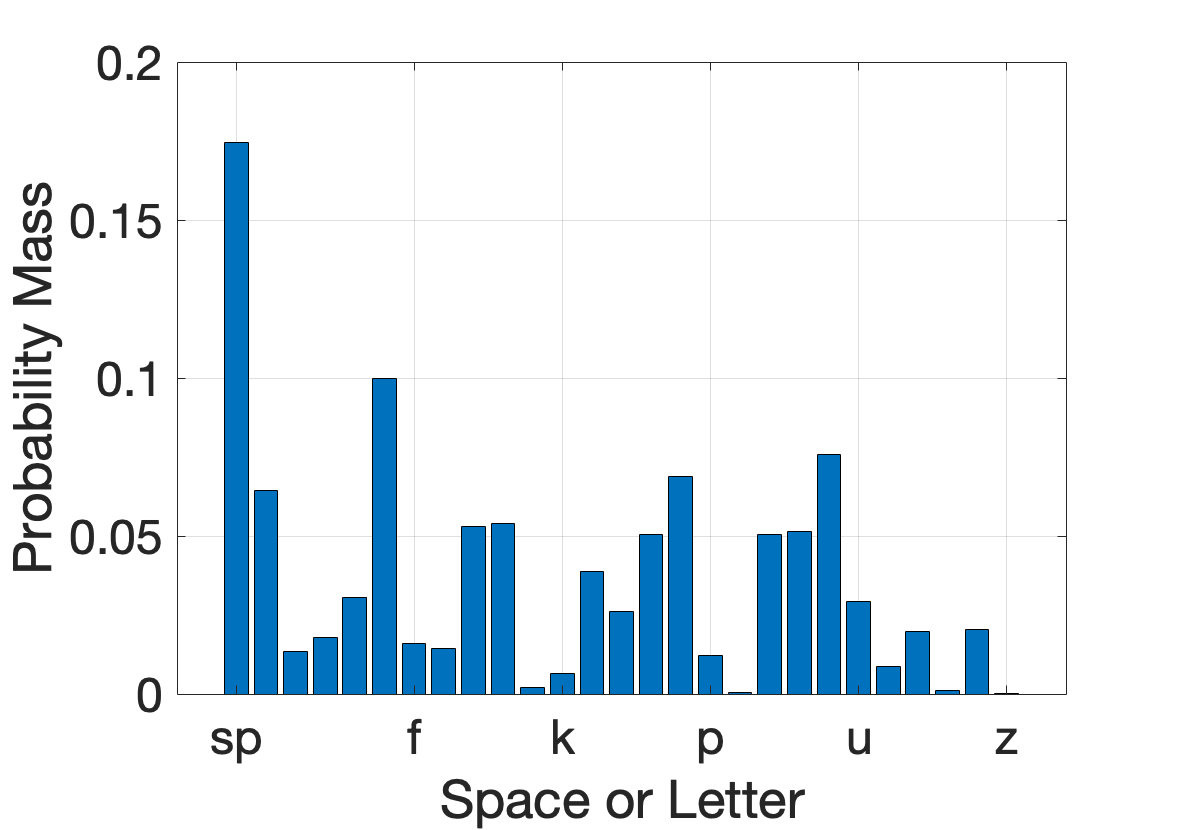
\includegraphics[width=2.9in]{pmf1char.png}
   (b) 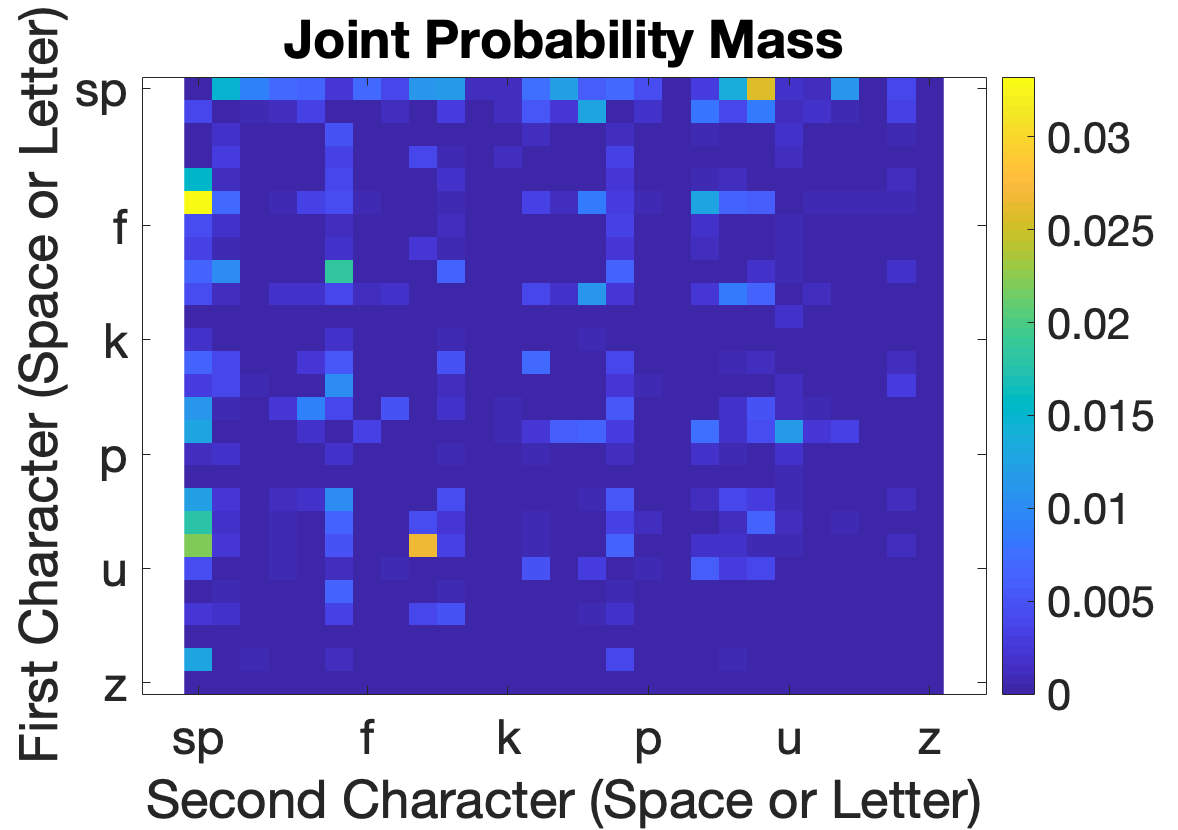
\includegraphics[width=2.9in]{pmf2char.png}
\end{array}$
  \caption{PMF of (a) single letters and (b) two-letter combinations (including spaces) in Shakespeare's \emph{Romeo and Juliet}.}
  \label{F:plotLetterPMF}
\end{figure*}

What is the entropy rate, $H$? Solution: For $N=10$, we have $H =
1.3$ bits/letter \cite[Section 6.2]{proakis2002communication}.}



\subsection{Source Coding Theorem}

The key connection between this mathematical definition of entropy
and the bit rate that we've been talking about all semester is given
by the source coding theorem.  It is one of the two fundamental
theorems of information theory, and was introduced by Claude Shannon
in 1948.

\Theorem{A source with entropy rate $H$ can be encoded with
arbitrarily small error probability, at any rate $R$ (bits / source
output) as long as $R>H$.  Conversely, if $R<H$, the error
probability will be bounded away from zero, independent of the
complexity of the encoder and the decoder employed.}{Proof: Using
\emph{typical sequences}. See Shannon's original 1948 paper.}

Notes:
\begin{itemize}
  \item Here, an `error' occurs when your compressed version of the
    data is not exactly the same as the original.  Example: B\&W
    images.
  \item $R$ has units of bits per source output.  A source output for audio, for example, would be one sample.  If we had audio at 44,000 samples/second, then $R(44\times 10^3)$ would give us the source bits/second.
  \item Theorem fact:  Information measure (entropy) times source output (sample) rate gives us a minimum bit rate .
  \item What is the minimum possible rate to encode English text (if you remove all punctuation and use only lowercase letters)?
  \item The theorem does not tell us how to do it -- just that it
    can be done if you are allowed infinite latency ($N$).
  \item The theorem does not tell us how well source encoding can be done if $N$ is not infinite.  That is, for a finite source, the rate may need
    to be higher.
\end{itemize}
